\chapter{Introduction}

As humans, we use cognitive skills to identify and localize objects around us. Those skills have been developed during our childhood and we are able to make good use of them for daily tasks such as car driving. For this particular use case we need to identify the different traffic signs and act upon them. We also need to estimate the location of people, cars and immovable objects around us to safely travel to our destination. More and more, computer systems assist us in our daily tasks by sensing the environment and taking appropriate actions. In the example of car driving, many car pilot systems are able to recognize traffic signs and will inform us when we are speeding. More advanced systems localize cars and pedestrians around us and will slow down our car when there's a risk of collision. Just as humans, computer systems need to be trained to recognize objects, but in the latter case, digital images of the real world will be used. We will be focusing on object localization, which is one of the functions a car pilot system requires.

To explain the \acrfull{mwsol} task, we will position it to the different object recognition tasks that exist. As neural networks are used to learn and perform object recognition tasks, we will discuss the main concepts and terminology required to understand next chapters. Then we briefly explain how computers can learn the object recognition task using those networks. After that, we introduce the concept of \acrlong{wsol} and its relationship with explainability. Finally we briefly look ahead at what is coming in the next chapters.

\section{Object recognition tasks}
Object recognition is a generic term covering a set of computer vision tasks for identifying objects in digital images. Fig. \ref{fig:object_recognition_tasks} shows the main tasks. From left to right: classification \cite{lecun1998gradient}, localization \cite{zhou2016cvpr}, object detection \cite{girshick2014rich}, instance segmentation \cite{He_2017_ICCV}. Classification aims to identify the main object portrayed in the image, i.e. 'cat'. Localization identifies the main object in the image and its location, indicated as the red bounding box in the figure. Object detection identifies every object and its location: A cat with a red bounding box and a dog with a blue bounding box. Instance segmentation classifies every pixel in an image and identifies the boundaries of objects. In this example the dog is marked with a blue mask and cat with a red mask.
\begin{figure}[ht]
    \begin{center}
    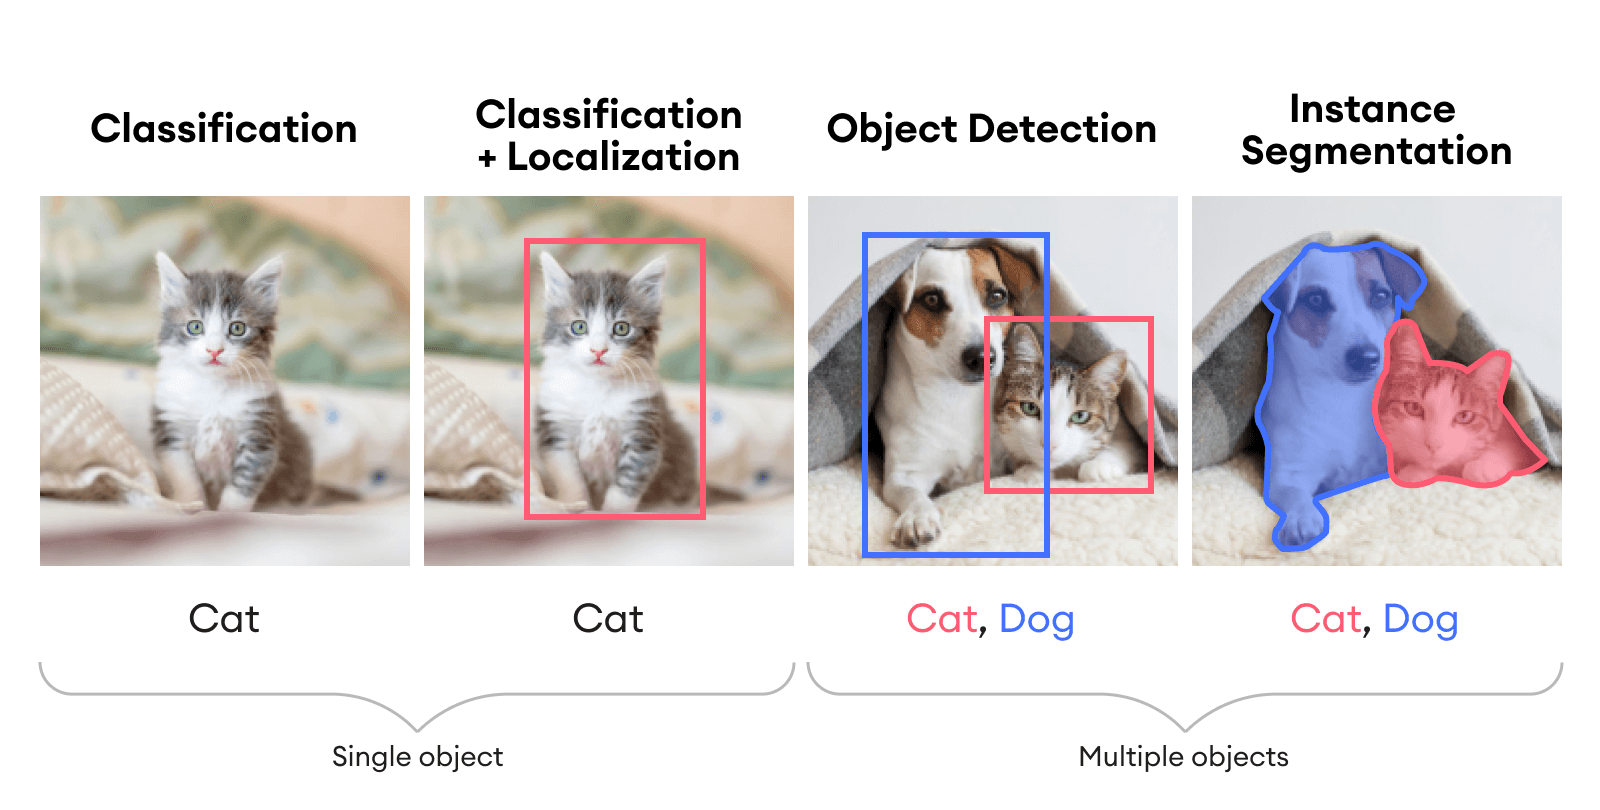
\includegraphics[width=\textwidth]{fig_object_recognition_tasks.png}
    \caption[Object recognition tasks]{
    Object recognition tasks.}
    \caption*{
    Source: \href{https://www.superannotate.com/blog/image-segmentation-for-machine-learning}{https://www.superannotate.com/blog/image-segmentation-for-machine-learning}}
    \label{fig:object_recognition_tasks}
    \end{center}
\end{figure}

\subsection{Image classification}
Image classification is a task that assigns a single class label to an image. So, an image classification algorithm takes as input an image with one or more objects and returns a class label prediction. For example, given an image depicting an animal, an image classification model would return one of the labels 'cat', 'dog, 'horse', etc. In the example of Fig. \ref{fig:object_recognition_tasks}, the model returns the class label 'cat'. It's important to notice that this task only recognizes an object of a specific class in an image, i.e. the object category the model is trained to identify. It doesn't return the location of an object within an image.

\subsection{Object localization}
it might be good to stress that here we start from the assumption that the object of interest (in the input image) has already being recognize and in this problem we are tasked with predicting its location (bounding box).

With object localization, we are able to identify the main subject and its location in an image. It's important to stress that this task starts from the assumption that the object of interest in the image has already been recognized, and that in the object localization problem, the task is to predict the location of the object. For this task, a model trained for classification, localizes the main object in that image by generating a bounding box surrounding that object. A bounding box is typically represented by two points: the top-left and bottom-right coordinates of the box. There is only one class label per image as the result of classification. As a consequence, object localization only recognizes objects of the same class. \acrfull{wsol} \cite{zhou2016cvpr} is an object localization task that only requires image-level labels to learn a model that can localize a single object in an image. In this work we define \acrfull{mwsol} as a \acrshort{wsol} task that has as goal to find a bounding box per object instance of the same image-level class in an image.

\subsection{Object detection}
Object detection is the task of identifying and localizing all objects in an image that a model has been trained for. It does so by assigning a bounding box and class label to each detected object. Hence, an object detection model takes as input an image with one or more objects and returns a set of bounding boxes and corresponding class labels.

\subsection{Instance segmentation}
Segmentation is a dense pixel-wise prediction task that classifies each pixel in an image. Instance segmentation distinguishes between multiple instances of the same class. Its output can be used for object counting, although it is not the goal of the task.
Consider an image with a cat and a dog as shown in Fig. \ref{fig:object_recognition_tasks}, then instance segmentation returns a segmentation map for each instance of a dog and a cat.

A related dense pixel-wist prediction task is semantic segmentation. This task classifies each pixel of an image, resulting in a segmentation mask per object class. Because of the single segmentation mask per object class, semantic segmentation cannot make the distinction between object instances of the same class.

\section{Artificial neural networks}
State-of-the-art object detection methods are implemented using an \acrfull{ann}. Here, we introduce the basic concepts and terminology of neural networks as we will use those terms further in this document. 

\subsection{Inspiration from real neurons}
Artificial neural networks are biologically-inspired models that attempt to mimic the functions of neurons in the brain. Neurons are the fundamental units of the brain and nervous system, the cells responsible for receiving sensory input from the external world, for sending commands to our muscles, and for transforming and relaying the electrical signals at every step in between.
\begin{figure}[ht]
    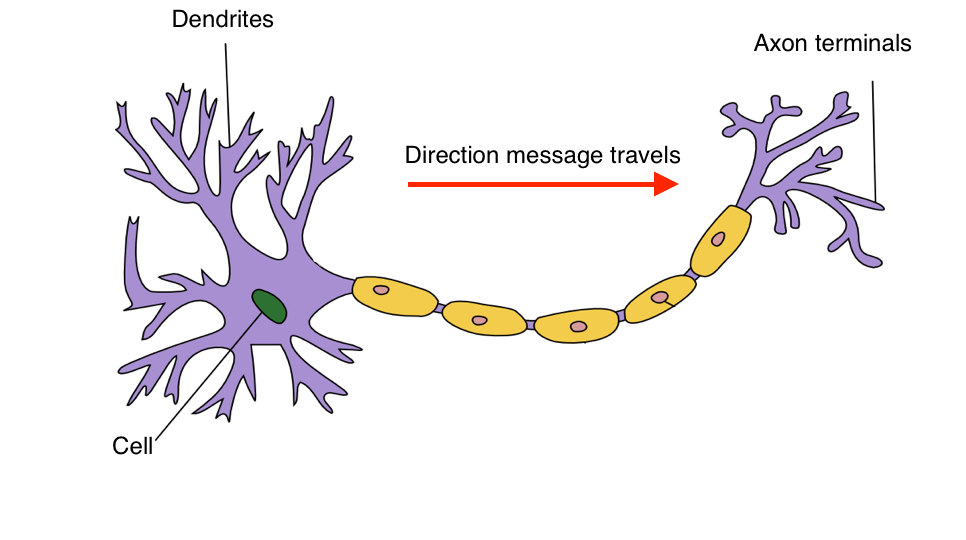
\includegraphics[width=\textwidth]{fig_neuron.png}
    \caption[Diagram of a biological neuron]{Diagram of a biological neuron.}
    \caption*{Source: \href{ https://medium.com/analytics-vidhya/mp-neuron-model-f4feb53c21a2}{https://medium.com/analytics-vidhya/mp-neuron-model-f4feb53c21a2}}
    \label{fig:neuron}
\end{figure}
Figure \ref{fig:neuron} illustrates the different parts of a biological neuron.
Each neuron acts as a computational unit, accepting input signals from other neurons via the dendrites and outputting signals through the axon terminals. Actions are triggered when a specific combination of neurons are activated.

\subsection{A computational model for an artificial neuron}
In computer science, we want to build artificial neurons that act as functions taking inputs and producing outputs. The perceptron \cite{rosenblatt1958perceptron, minsky2017perceptrons}, illustrated in Fig. \ref{fig:perceptron}, is the basic building block of a \acrfull{nn}. It takes weighted input values, performs a mathematical calculation and produces output. It is also called a unit or node.
\begin{figure}[ht]
    \begin{center}
    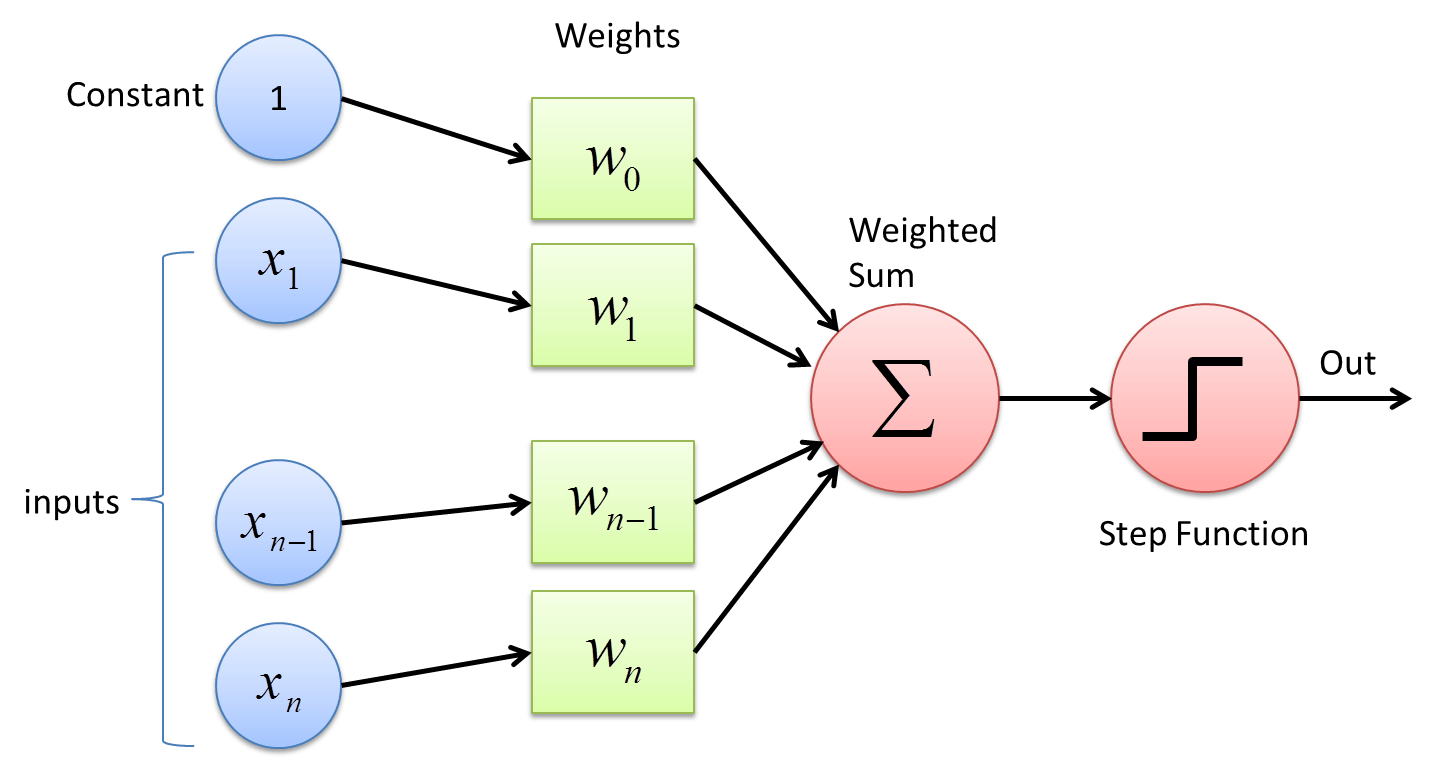
\includegraphics[width=0.8\textwidth]{fig_perceptron.png}
    \caption[Perceptron]{Perceptron.}
    \caption*{Source: \href{https://deepai.org/machine-learning-glossary-and-terms/perceptron}{https://deepai.org/machine-learning-glossary-and-terms/perceptron}}
    \label{fig:perceptron}
    \end{center}
\end{figure}
A neuron consists of following building blocks:
\begin{itemize}
    \item \textbf{Input} is the data passed to a neuron.
    \item \textbf{Weights} explain the strength (degree of importance) of the connection between any two neurons.
    \item \textbf{Bias} is a constant value added to the weighted sum of input values. It is used to accelerate or delay the activation of a given node.
    \item \textbf{Activation function} is used to introduce non-linearity into a \acrshort{nn}. The perceptron activation function is a step function limiting the output value from 0 (when the neuron doesn't activate), to 1 (when the neuron activates).
\end{itemize}
As the perceptron output produces either 0 or 1, this model is only capable of binary classification of the input. It divides the input in two classes. To learn the function that can classify input into the correct class, the weights are tuned over time. This process of tuning is called training of the model: We start with some initial value of the weights and those values get updated to minimize the error between the function output and the expected output.

\subsection{A network of neurons}
The previous model is only capable of binary classification. However, we can perform multi-class classification by extending the network. A \acrfull{nn} is made of several neurons stacked into layers. For an n-dimensional input, the first layer (also called the input layer) will have a number of input nodes and the final output layer will have a number of output neurons. All intermediate layers are called hidden layers. The first layer, the input layer, performs no computation except to pass the input values. For this reason, when counting the number of layers in a \acrshort{nn}, we ignore the input layer. Fig. \ref{fig:neural_network} shows a neural network with 2 hidden layers and a single output neuron. 
\begin{figure}[ht]
    \begin{center}
    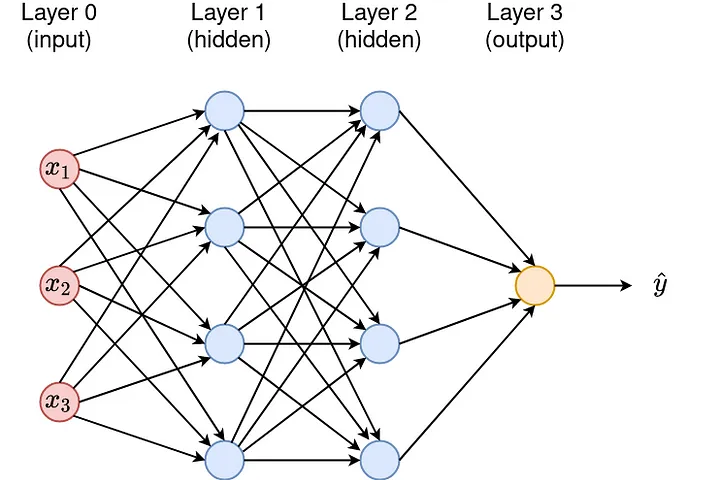
\includegraphics[width=0.8\textwidth]{fig_neural_network.png}
    \caption[Neural network]{Neural network.}
    \caption*{Source: \href{https://towardsdatascience.com/the-basics-of-neural-networks-neural-network-series-part-1-4419e343b2b}{https://towardsdatascience.com/the-basics-of-neural-networks-neural-network-series-part-1-4419e343b2b}}
    \label{fig:neural_network}
    \end{center}
\end{figure}

For more complex problems, neural networks with more layers are required. The number of layers in a \acrshort{nn} determines the depth of the network. A neural network with many hidden layers is called a \acrfull{dnn}. 
A \acrfull{mlp} \cite{hornik1989multilayer} is a special case of a \acrshort{nn}. In \acrshort{mlp}, all nodes are densely-connected, i.e. each neuron is connected to all nodes in the previous layer. These layers are also called fully connected layers. The \acrshort{nn} in Fig. \ref{fig:neural_network} is called a \acrshort{mlp} or feed-forward network. Models that are capable of classifying input to more than two classes will have as many outputs as there are classes.

\section{Convolutional neural networks}
There are many different types of neural network architectures, each with their own benefits. A \acrfull{cnn} is used a lot for object recognition tasks because it provides some advantages over feed-forward networks due to the characteristics of visual data.

\subsection{Visual data characteristics}
The method we use to recognize objects should not be overly concerned with the precise location of the object in the image. Let's take an example of the game “Where’s Waldo in Fig. \ref{fig:where_is_wally} \cite{zhang2021dive}. Despite Waldo's characteristic outfit, it can be difficult to locate him, due to the large number of distractions. However, what Waldo looks like does not depend upon where he is located. 
\begin{figure}[ht]
    \begin{center}       
    
\includegraphics[width=0.8\textwidth]{fig_where_is_wally.jpeg}
    \caption[An image of the “Where’s Waldo” game]{An image of the “Where’s Waldo” game.}
    \caption*{Source: \href{https://d2l.ai/chapter\_convolutional-neural-networks/why-conv.html\#invariance}{https://d2l.ai/chapter\_convolutional-neural-networks/why-conv.html\#invariance}}
    \label{fig:where_is_wally}
    \end{center}
\end{figure}

Convolutional neural networks are suited for object recognition because they meet some desired properties:
\begin{enumerate}
    \item \textbf{Translation invariance}. In the earliest layers, the network should respond similarly to the same object, regardless of where it appears in the image. 
    \item \textbf{Locality}. The earliest layers of the network should focus on local regions.
    \item \textbf{Compositionality}. As we proceed, deeper layers should be able to aggregate local representations to make predictions at image level.
\end{enumerate}

An \acrshort{mlp} is not suited for computer visual tasks because every neuron is fully-connected to all neurons at the previous layer meaning that every neuron in the early layers looks at the complete image. Hence an \acrshort{mlp} doesn't have the locality and translation invariance properties.

\subsection{The convolution operation}
Where a neuron in \acrshort{mlp}s is fully-connected to all neurons in the previous layer, neurons in \acrshort{cnn}s are computed using convolutional operations. Fig. \ref{fig:convolution} shows how this operation works for two-dimensional data representation. In this example we have an input image with height and width of 3. The kernel has height and width of 2. The kernel, also called a filter, will slide like a window over the input from left to right and from top to bottom. At each position, the input contained in the window and the kernel are multiplied element wise and the results are summed yielding a single scalar value. This result gives the value of the output at a specific location. Here, the output has a height and width of 2.
\begin{figure}[ht]
    \begin{center}       
    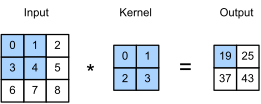
\includegraphics{fig_convolution.png}
    \caption[Two-dimensional convolution operation]{Two-dimensional convolution operation.}
    \caption*{Source: \href{https://d2l.ai/chapter\_convolutional-neural-networks/conv-layer.html}{https://d2l.ai/chapter\_convolutional-neural-networks/conv-layer.html}}
    \label{fig:convolution}
    \end{center}
\end{figure}

The input and output neurons are called features. The output features are the weighted sums (with the weights being the values of the kernel itself) of the input features. The example in Fig. \ref{fig:convolution} shows a convolution for a single-channel input layer. For RGB images, the input would have three channels. In that case the kernel would be 3-dimensional, covering all channels of the input layer. The kernel's values are used to detect certain characteristics of an object, like edges or patterns. Typically, each hidden convolutional layer has multiple channels, and thus also multiple kernels to match the number of hidden layers. For large kernels and many successive layers of convolutions, it's unfeasible to design kernels by hand. The kernel weights will be learned when training a \acrshort{cnn} model with images.

To understand certain concepts that are used further in the document, we now introduce terminology that is illustrated Fig. \ref{fig:receptive_field}.

\textbf{Feature map}. A feature map is the output of the convolution operation. When a kernel $K_1$ is applied to an input in a convolutional layer, a feature map $F_1$ is produced. When another kernel $K_2$ is applied to the same input, another feature map $F_2$ is produced. A feature map is also called an \textbf{activation map}.

\textbf{Receptive field}. A receptive field is the portion of the input image that is used to compute the activation of a neuron in a feature map.

\begin{figure}[ht]
    \begin{center}       
    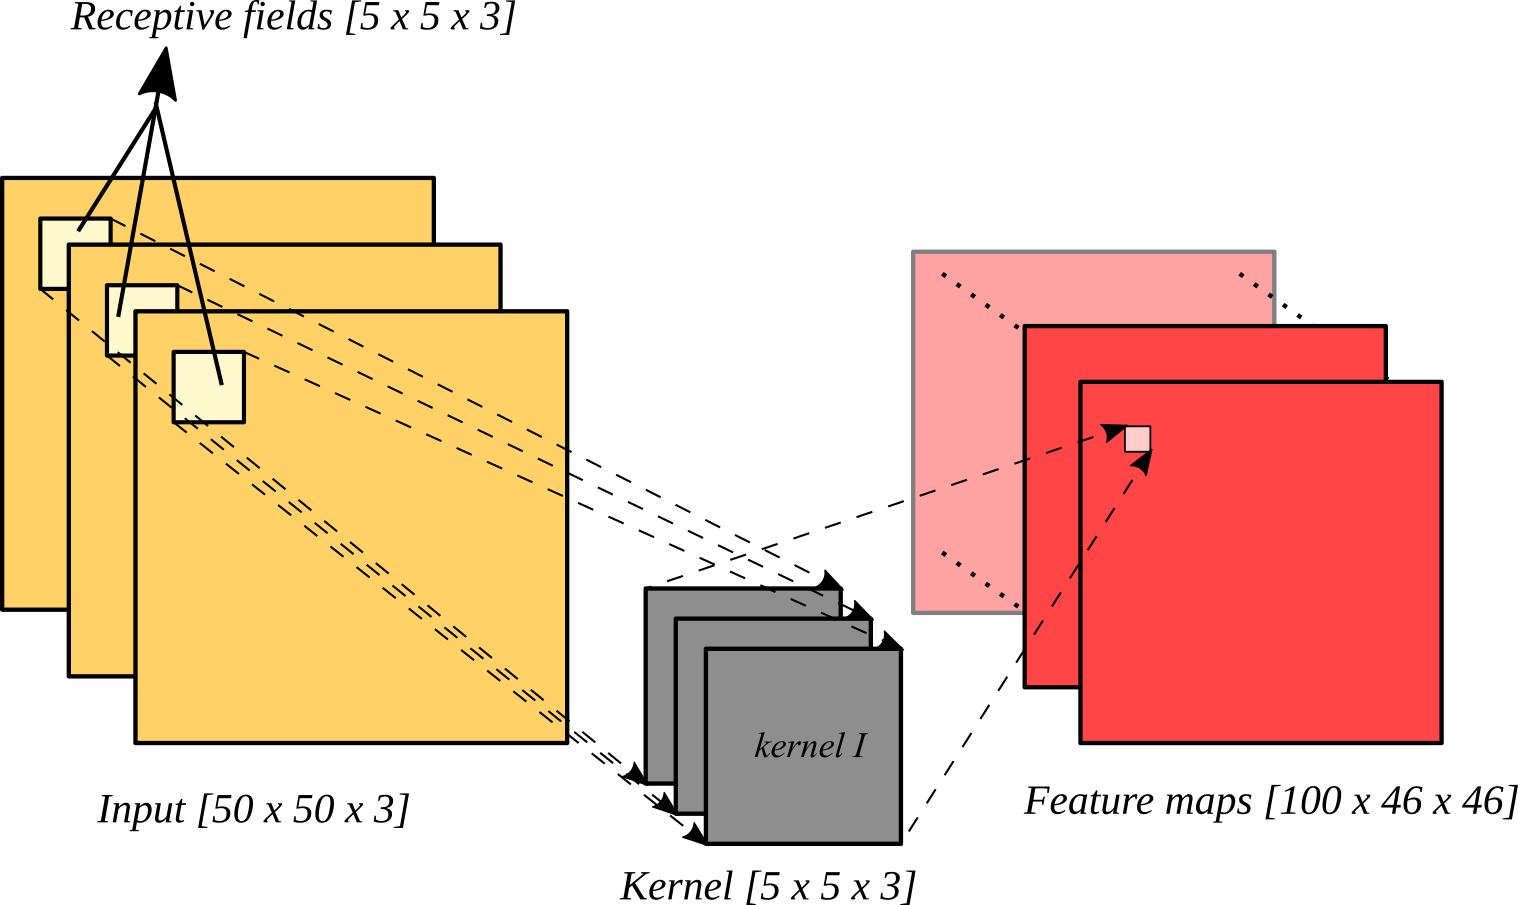
\includegraphics[width=0.8\textwidth]{fig_receptive_field.png}
    \caption[Receptive field and feature maps]{Receptive field and feature maps.}
    \caption*{Source: \href{https://ai.stackexchange.com/questions/8701/what-is-the-difference-between-a-receptive-field-and-a-feature-map}{https://ai.stackexchange.com/questions/8701/what-is-the-difference-between-a-receptive-field-and-a-feature-map}}
    \label{fig:receptive_field}
    \end{center}
\end{figure}

In the example illustrated in Fig. \ref{fig:receptive_field}, the output feature map is a 2-dimensional matrix of shape 46×46. There are 100 feature maps (so 100 kernels were applied to the input image). The receptive field of a neuron is a 3-dimensional sub-region of the image of shape 5×5×3. In this case, the kernel has the same depth as the input image.

A we go deeper into a \acrshort{cnn}, the receptive field of neurons increases. This is because the output feature map of a convolutional layer is the input of the next layer. That next layer will produce feature maps in which neurons will cover a larger receptive field because it covers multiple neurons of the previous layer.

\subsection{Pooling}
To answer the question whether an image is of a certain class, a model should learn a global feature representation of the input. By gradually aggregating information into coarser feature maps, we can reach that goal. Pooling layers are used for this task. They actually serve two purposes: Mitigation of the sensitivity of convolutional layers to location, and spatial downsampling of representations.

\begin{figure}[ht]
    \begin{center}       
    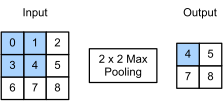
\includegraphics[]{fig_pooling.png}
    \caption[Maximum pooling]{Maximum pooling.}
    \caption*{Source: \href{https://d2l.ai/chapter\_convolutional-neural-networks/pooling.html}{https://d2l.ai/chapter\_convolutional-neural-networks/pooling.html}}
    \label{fig:pooling}
    \end{center}
\end{figure}

Fig. \ref{fig:pooling} shows the concept of pooling. As with the convolutional operation, we can think of a pooling window, starting from the upper-left of the input and sliding across the input from left to right and top to bottom. At each location, pooling computes the maximum or average value of the input in the window, depending on whether maximum or average pooling is employed. In the example of Fig. \ref{fig:pooling}, the $3 \times 3$ image is fed to the $2 \times 2$ pooling layer and the resulting output is a $2 \times 2$ feature map.

When the pooling window has the same size as the input, it is called a global pooling layer and the output will be a single neuron. In case an average operation is applied, we refer to this layer as a \textbf{\acrfull{gap}} layer \cite{lin2013network}.


\subsection{The network architecture}
Depending on the task to solve, many different types of \acrshort{cnn} architectures exist, but they all share some basic building blocks. A network architecture used for the image classification task is shown in Fig. \ref{fig:cnn_arch}. There are two major parts in the architecture:
\begin{itemize}
\item \textbf{Feature extractor.} This part contains all convolutional layers and is used to detect the features that are relevant for the recognition of the main object portrayed in the input image. These features will serve as input to the classifier.
\item \textbf{Classifier.} This part of the network has fully-connected layers and takes as input the features from the feature extractor, and produces a   prediction for the class of the input image.
\end{itemize}
\begin{figure}[ht]
    \begin{center}       
    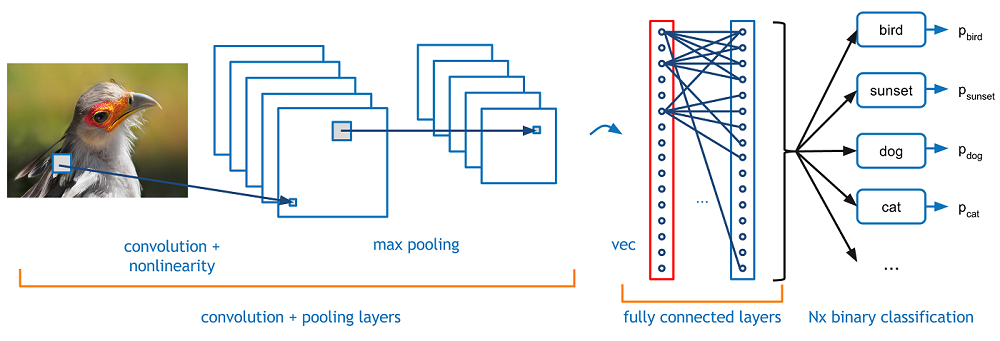
\includegraphics[width=\textwidth]{fig_cnn_arch.png}
    \caption[A CNN architecture for image recognition]{A CNN architecture for image recognition.}
    \caption*{Source: \href{https://towardsdatascience.com/covolutional-neural-network-cb0883dd6529}{https://towardsdatascience.com/covolutional-neural-network-cb0883dd6529}}
    \label{fig:cnn_arch}
    \end{center}
\end{figure}

\section{Learning the task}
Assume there's a perfect hypothetical function that can classify images correctly. As we don't know that function, we approximate that function using a neural network model to predict the outcome of that hypothetical function. We train the model using images and class labels to verify whether the predictions made by the model are correct. A loss function will express the error between the predictions and the actual labels, also known as ground truth labels.

A neural network implements the approximated function using many weights, which need to be trained to approximate the hypothetical function as close as possible. The training of these weights is typically done by minimizing the loss function. To minimize that loss function, the gradients of that function with respect to the network weights are computed, to move the loss function towards its minimum by updating the weights with their gradients. This process is called \acrfull{sgd} \cite{amari1993backpropagation}. Fig. \ref{fig:learning} illustrates this process for the loss function $J(w)$ in function of the weight $w$. The gradient of $w$ is computed as the partial derivative of $J(w)$ with respect to $w$. By updating $w$ in the opposite direction of its gradient, we move the loss function $J(w)$ towards its local minimum.
\begin{figure}[ht]
    \begin{center}       
    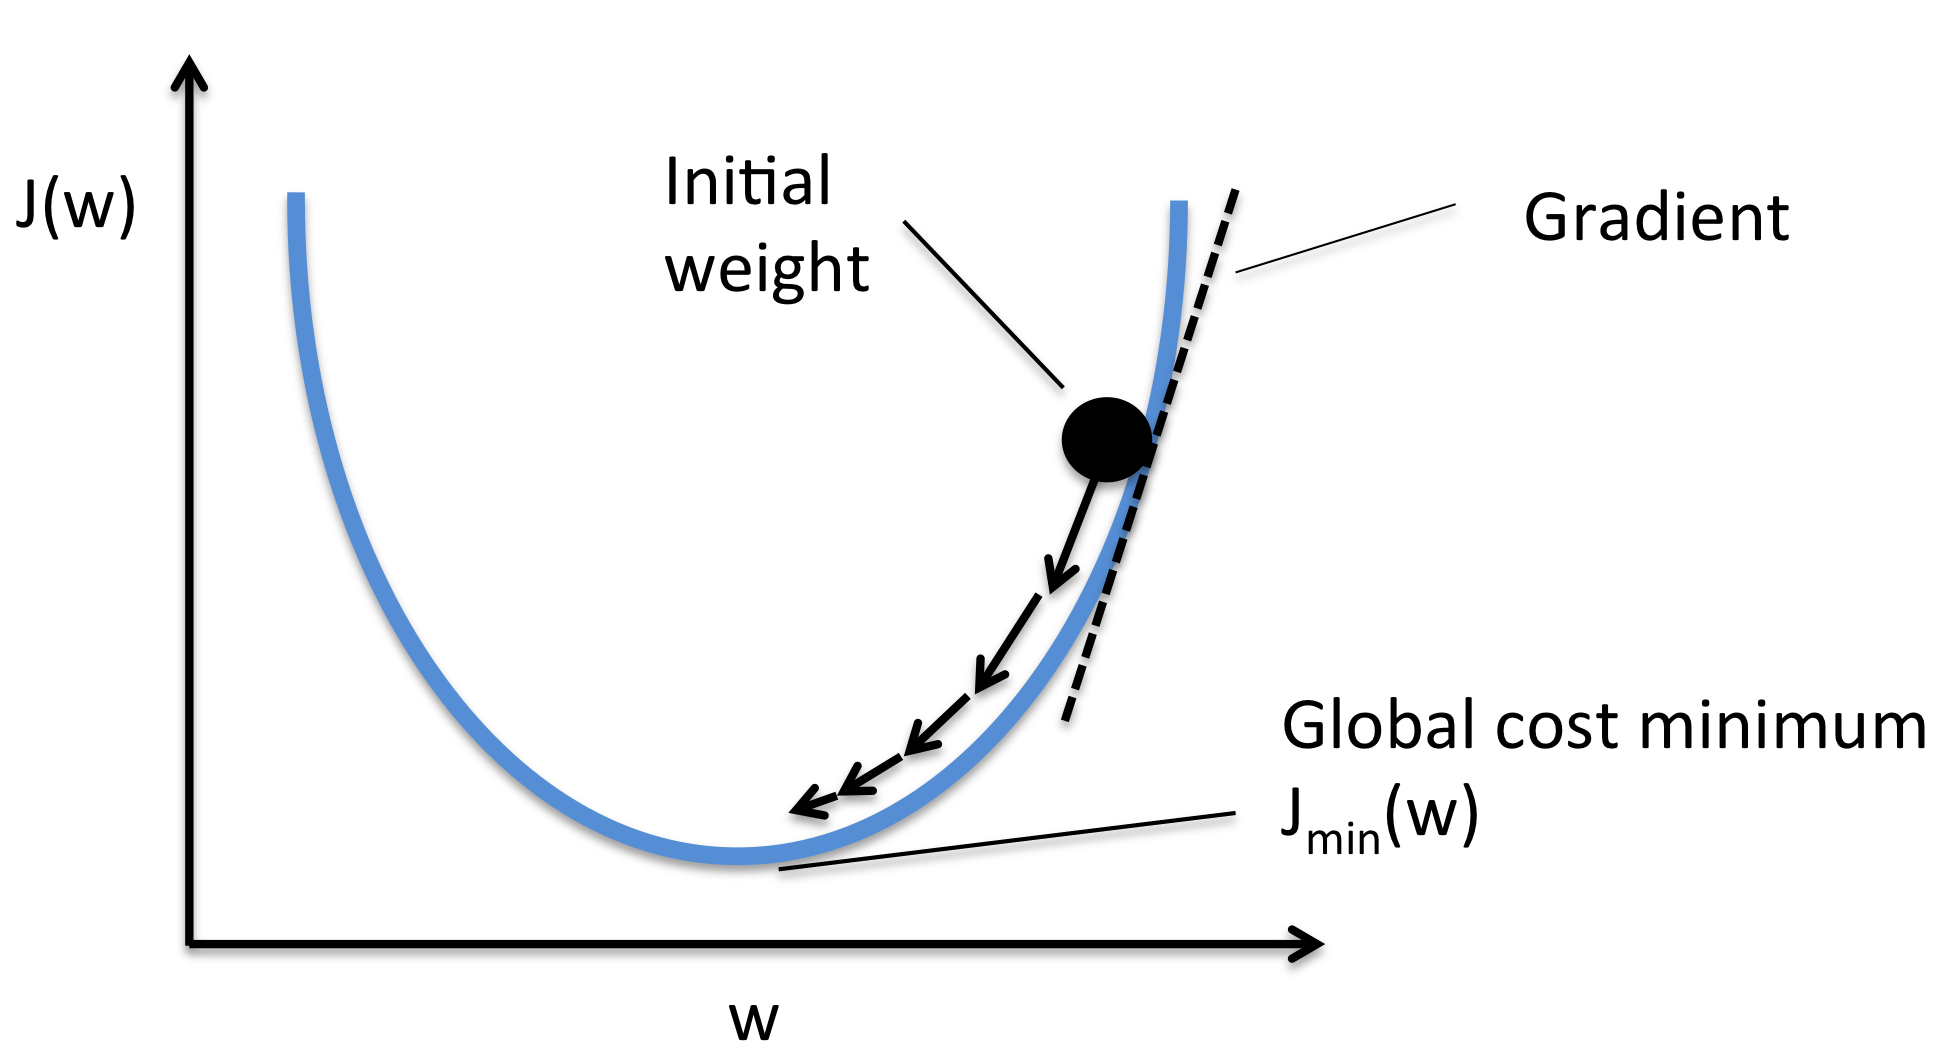
\includegraphics[width=0.8\textwidth]{fig_learning.png}
    \caption[How neural networks learn weights]{How neural networks learn weights.}
    \caption*{Source: \href{https://paperswithcode.com/method/sgd}{https://paperswithcode.com/method/sgd}}
    \label{fig:learning}
    \end{center}
\end{figure}

\section{Weakly supervised object localization}
Traditional supervised tasks like object detection require bounding box annotations to learn the task of localizing objects. These bounding box annotations are collected by human labeling of images with bounding boxes, which is a costly and error-prone task. Where object detection recognizes all object instances and their classes, object localization's task is to predict the location of the main object of interest in an image, assuming that the object of interest has already been recognized.

In contrast to object detection, \acrshort{wsol} is an object localization task that trains a model by only using image-level labels. Hence the term weakly: Training requires image-level class labels but no object-level class labels or localization bounding boxes. Because costly human labeling of object locations is not required, \acrshort{wsol} research has gained significant momentum \cite{zhou2016cvpr, selvaraju2017grad, chattopadhay2018grad, wang2021minmaxcam, wang2020score, choe2020evaluating}.

The baseline \acrshort{wsol} method is \acrfull{cam} \cite{zhou2016cvpr}. This method trains a model for the classification task and uses learned features that are activated on the most discriminative parts of an object to localize an object of a specific class. This focus on the most discriminative parts is a limitation of the \acrshort{cam} method, as it doesn't cover the complete object. New \acrshort{wsol} research \cite{selvaraju2017grad, chattopadhay2018grad, wang2021minmaxcam, wang2020score, choe2020evaluating} focuses on overcoming the limitations of the baseline \acrshort{cam} method. As the CAM-based family of methods represents a main body of research for \acrlong{wsol}, we will use a specific list of CAM methods in this project. The relevant methods will be discussed in chapter \ref{ch:related_work} and \ref{ch:methodology}. 

\subsection{WSOL and explainability}
%(similarities and differences between wsol and explainability)
WSOL methods share similarities with model explainability. They both analyse which image pixels lead to image classification results. On the other hand, they both serve different goals.
Model explainability is used to visually explain why a model predicts a certain label by capturing the discriminative features. Typically these features cover only parts of an object of interest. In contrast, the goal of \acrshort{wsol} is to localize the full extent of an object of interest.

Certain CAM-related techniques are mainly used for explainability, i.e. they are used to visually explain why a model predicts a certain class label for an image. Some of these methods indicate the ability to detect multiple object instances of the same class in an image and show promising results in qualitative experiment results \cite{wang2020score}.

\subsection{WSOL evaluation}
Many \acrshort{cam} papers report performance improvements over the baseline \acrshort{cam} method. Choe \textit{et al.} \cite{choe2020evaluating} criticize that \acrshort{cam} methods lack a unified definition of the \acrshort{wsol} task and the authors propose a new localization evaluation protocol. A problem is that \acrshort{wsol} has not been tested for localization of multiple object instances of the same class, and thus, current \acrshort{wsol} evaluation metrics are not sufficient to measure localization of multiple object instances. Given that multiple-instance localization hasn't been tested, it is interesting to evaluate it. 

\section{Our contribution}
The research question for us is:

\begin{center}
\textbf{\textit{Can we use CAM-based methods to evaluate and improve localization of multiple object instances of the same class within images for the \acrshort{wsol} task?}}
\end{center}

Therefore, we propose an evaluation protocol for localization of multiple object instances of the same class by enhancing existing evaluation metrics \cite{choe2020evaluating}, to measure multiple-instance localization performance.  We then benchmark existing CAM-based methods for multiple-instance localization. Finally, we investigate improvements for the \acrshort{mwsol} task, by using an iterative bounding box extraction method. Location information of object instances localized in previous iterations, is used to mask the location of those object instances in images. These masked images are then used to find the location of object instances missed during previous iterations.

\section{Looking ahead}
In chapter \ref{ch:related_work}, we discuss the \acrshort{wsol} related research work, on which we base our work on: More specifically the family of \acrshort{cam} methods and evaluation methods that we will use to benchmark multiple-instance localization. We will briefly point to \acrshort{wsol} work that is non-\acrshort{cam} related. 

The methodology used for evaluating \acrlong{mwsol} is explained in detail in chapter \ref{ch:methodology}. We describe the neural networks chosen for implementing the object localization models, the datasets for training the models and the \acrshort{cam} methods for object localization. We define enhancements of existing \acrshort{wsol} metrics required to evaluate localization of multiple instances and we explain an improvement strategy for localizing multiple instances.

We describe the results of our experiments in chapter \ref{ch:experiments}. For each method the computational complexity and localization performance are provided. Chapter \ref{ch:discussion} provides a detailed discussion of the experiment results. Our conclusions on \acrshort{mwsol} are explained in chapter \ref{ch:conclusion}.